\cleardoublepage
\counterwithout{figure}{section}
\counterwithout{table}{section} 
\counterwithout{equation}{section}
\counterwithin{figure}{chapter}
\counterwithin{table}{chapter} 
\counterwithin{equation}{chapter}


\chapter{Introduction}
\label{sec:problemstellung}
 Only in Germany more than 1 Million teeth are replaced annually. The replacement procedure is accomplished with an implantation of the tooth replica to provide the aesthetics and the function of the natural tooth. Ancient Egyptians used tooth shaped ivory to regain the function of the missing teeth. Today the technology has evolved to a point where the dental replacement for a single tooth is an assembly of three parts, which  are to be seen in Figure 1.1. The implant is the part which is screwed to the lower jaw bone (mandible) and anchors the whole replacement assembly to the chin. The preferred materials used for the implant are titanium in the EU and tantalum in the US. The enhanced osseointegration of the porous implant material surface, biocompatibility of the ceramic interface,which is formed due to the surface oxidation a Young's Modulus, which is similar to the human bone are the main reasons for titanium and tantalum to be the prime materials for this purpose. The abutment takes on the task of a fitting  for the crown and is made of the same material as the implant.
  \begin{figure}[h]
 	\centering
 	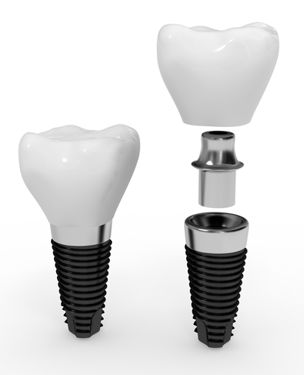
\includegraphics[width=0.4\textwidth]{grafiken/implant.png}
 	\caption{Single tooth replacement}
 	\label{fig:implant}
 \end{figure} 
 
 The crown of the tooth replacement is the part which imitates the visual qualities of the tooth. There are several materials, which a crown can be made of or assembled from. The most popular crown material dominating the market is the Yttria-stabilized zirconia (YSZ), which has a cubic fluorite crystal structure and is going to be referred as zirconia in the frame of this thesis. However, zirconia in its pure form is a plain white material with high translucency. In case of single tooth replacement the newly implanted crown would be absurdly white when compared to the neighboring teeth. Even when a full chin dental replacement is conducted, it is abnormal to have a full set of plain white teeth without any shading. This situation makes it a necessity to preprocess the crowns to match the neighboring teeth or another natural shade of choice in case of a fully monolithic replacement. Dentist are using a shade guide seen in the figure \ref{fig:shadeguide} for a side-by-side comparison to determine the color and the shade of the teeth. One can observe that there are 4 color groups A, B, C and D which are referred as orange-brown, yellow, grey-brown and red respectively \citep{vita}. Each of these colors have shades ranging from 1 to 4. Even though the shades are coded with the numbers from 1 to 4 with increments of 0.5 a total analogue shade acquisition is possible. The number 1 represents the shade with the least and 4 with the most saturated tone for each color.
 \newline
 \begin{figure}[h]
 	\centering
 	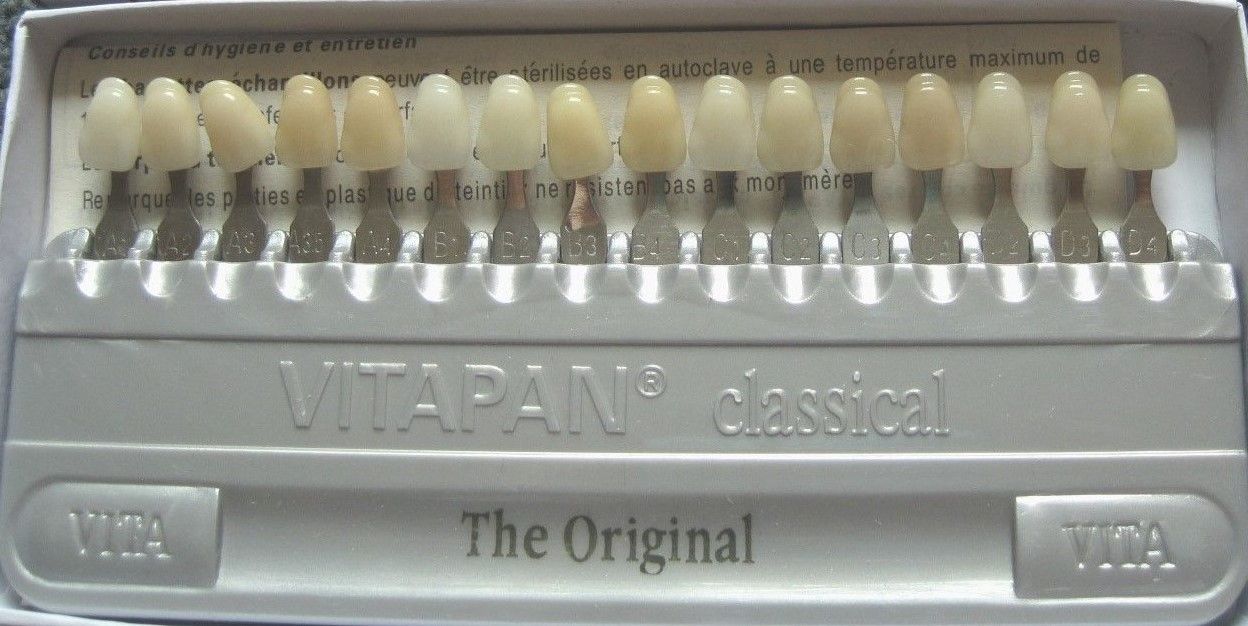
\includegraphics[width=0.9\textwidth]{grafiken/shadeguide.jpg}
 	\caption{Vitapan Shadeguide}
 	\label{fig:shadeguide}
 \end{figure}  
 


\chapter{State of the Research}
\label{sec:stand_forschung}

Addressing the shading process of the dental zirconia-based ceramics as a combined procedure of drop generation, dispersion of the ink within the porous material and post sinter generation of the color below the surface of the porous material, it can be said that the quantitative coloring process of the dental crowns is an uncharted area for the scientific researches in the present-day. There have been some research made in the fields concerning the absorption of the liquid by materials presenting a porous inner structure and permeable surface conditions. How the liquid is distributed inside the material, what are the effects of the pore sizes, forms and distributions is investigated by various teams from all around the world for a variety of liquids and porous materials. 



\section{Structure of the Porous Medium}

The crystallographic state of zirconia depends on the temperature under atmospheric pressure. Until reaching a temperature of {1170\textdegree} Celcius the crystallographic structure shows a monoclinic symmetry. After that temperature the structure can be defined as tetragonal until {2370\textdegree} C , which afterwards becomes cubic up to the melting point. The volume of the material increases about 4.5\% during the transformation from tetragonal to monoclinic phases, which is enough to cause a crack induced failure. This evitable transformation begins at about {950\textdegree} C while cooling down and the only way to stabilize the tetragonal structure is creating CaO, MgO, $Y_{2}O_{3}$ or $CeO_{2}$ oxides inside the structure to keep the tetragonal formation  at room temperature, which eliminates the crack induction and therefore the structural failure of the material parallel to an enhanced toughness. \citep{denry2008state}

On a different aspect, some research has been conducted about the effect of the coloring process on the structural strength of the zirconia. In the research of Shah et al. coloring zirconia with cerium acetate mixtures with a maximum ink weight ratio of 5\% provided a distinctive shade and did not cause a mechanical disadvantage. However, the ratios above 5\% have decreased the mechanical properties while not increasing the shading level significantly. The paper also includes data for case where the coloring process is conducted using cerium chloride and bismuth chloride. For both cases 1\% coloring agent was the limit, if the flexural strength was to be conserved. The low temperature degradation was also observed in the frame of the paper, which did not show any co-dependence with the coloring solution.\citep{shah2008effect}

\section{Ink Distribution and Infiltration Time}
In 2016 Lee et al. have investigated the absorption behavior of water drops impinging porous stones experimentally and numerically. The investigation includes the phases from spreading to evaporation for a water droplet considering the absorbed amount of the droplet during the depletion and spreading of the humidity within the manner depending on time for three porous materials. Quantitative measurements of the water absorption for the materials are conducted with high-speed imaging and neutron radiography methods during the time range from the impact moment to the end of the spreading phase after absorption. Neutron radiography shows a high resolution quantitative distribution of absorbed water. During the first contact and deposition on the surface the droplets do not exhibit a wetting behavior.  As soon as the droplet acquires its maximum diameter on the surface, it gets fixed and the contact angle with the surface remains constant as long as the droplet is not drained by the stone. The absorption behavior doesn’t have the same attributes throughout the whole process. At the beginning the material shows a contact resistance blocking the absorption, which is associated with the entrapped air beneath the area encapsulated by the borders of the water droplet. In the second phase the encapsulated air finds a way to diffuse away so the capillary flow takes place flawlessly until the total disappearance of the droplet on the surface is observed. The experimental data shows accordance to the phases of the numerical model for water flow inside the unsaturated porous material. The collision velocity has a huge effect on drop spreading on the surface and impregnation, but not so much on the distribution of the water after the initial absorption. The absorption and distribution rates are highly relevant to the capillary structure of the stones.\citep{lee2016absorption}


Pecho et al. have conducted experiments to analyse the optical behaviour of dental zirconia and dentin in comparison utilizing Kubelka-Munk theory. The results show that the current zirconia materials alone could not satisfy the luminous transmittance of the natural dentin so an additive application of masking is required to reach an approximate to the natural tooth.\citep{pecho2015optical}

The infiltration time of the porous medium was formulated by Markicevic et al. in 2009 as:

\begin{equation}\label{eq:InfTime}
t_{in}=\kappa \cdotp {\frac{\mu \cdotp r{_0}^{1.85}}{\sigma \cos({\theta})\varPhi^{0.38}}}
\end{equation}

\bigskip

$t_{in}$ defines the infiltration time and depends on the parameters $\kappa$ , which is the permeability constant of the medium and $\mu$ the kinematic viscosity of the fluid. The initial drop radius is symbolized by $r_{0}$. $\theta$ stands for the initial contact angle after the impact of the droplet on the surface. The $\sigma$ in the denominator is the surface tension of the liquid. The higher the surface tension is the harder it is for the liquid to wet the surface of the material because of the increased contact angle and hardened impregnation capability. The last dependency of the infiltration time is  the $\phi$ constant for the material, identifying the porosity level of the material. \citep{markicevic2009infiltration}

Stratov et al. have provided experimental results regarding  the spreading phases of silicon oil droplets utilizing capillary forces over different permeable layers and observing the diameters of the droplets and wetted areas over time. They have divided the depletion into two phases, of which the first one is defined by the time to reach the maximum diameter for the drop base and the second one is identified by the reduction of the drop base while the depletion takes place. The findings of the experiments show that the different oils on the different porous materials with similar porosity and mean pore dimensions. showed similar spreading characteristics on a different time scale and the contact angle remained constant throughout the second stage.\citep{starov2002thick}

The dispersion behavior of liquid drops inside porous media which are previously saturated with the identical liquid are examined in the work of Starov et al. The study was conducted both theoretical and experimental perspectives. The spreading of a liquid on a dry solid medium is governed by a power law and it is shown that the same power law applies to the case with saturated medium. The liquid flow within the porous medium is modeled using the Brinkman’s equations. The effective lubrication and the liquid exchange between the drop and the porous medium are found to have equal significance through which the drop dispersion equation is generated. \citep{starov2002saturated}
\bigskip

\begin{equation} \label{eq:SpreadingDia}
L=L_0 (1+10(\frac{4}{\pi})^3 \frac{V^3 \gamma}{L_0^{10} \mu}\omega t)^{0.1}
\end{equation}
\bigskip

The formula \ref{eq:SpreadingDia} shows the parameters which define the diameter of the covered spot by a deployed drop on the saturated surface of the porous material. $L_0$ V are the measured initial diameter and volume of the drop. $\omega$ is defined as the effective lubrication coefficient and has to be acquired experimentally for each porous medium and impregnating liquid pair. The t as the last parameter of the equation stands for the time. 

According to Hapgood et al. the properties of the porous medium, such as its porosity, the size and the orientation of the pores and the chemical properties of the surface affect the impregnation and the dispersion behavior of the drops. The Washburn equation is employed by multiple authors to generate a model. These models are grounded on the existence of cylindrical capillaries lying parallel to each other. The Washburn equation describes the behavior of the drops by stating that the wetting is induced by capillary pressure while the viscous dissipation of the flow causes resistance to the dissipation.

The amount of time it takes for a drop to diffuse completely in the porous substrate, until there remains no more liquid on the surface is defined as the drop penetration time, also called as the wicking time.

The fact that the parallel capillary pores assumption not being suitable for direct implementation for powder beds brings about a major disadvantage. To overcome this problem, the Kozeny approach, which utilizes an effective pore size based on the properties of the powder, is widely applied. The 3D velocity components of a Newtonian fluid were measured in the porous medium model under the assumption that the flow is steady, viscous and incompressible. Glass rods with diameters of 3mm were used for building the models of porous media. Two of the velocity components were measured with a laser Doppler anemometer while the  continuity equation is integrated to calculate the third component. The main aim was to observe how the viscous drag, inertial flow field and eddy losses in the porous medium affect the flow. The study revealed a laminar and stable  flow, which brings along the conclusion  that a micromixing of the fluid does not exist. In addition, high values of viscous drag coefficients lead to non-existent inertial flow effects.

Although the vertical and lateral velocity fields are observed  to have positive and negative  flow fields, the bulk direction flow fields do not have negative velocity fields. At the top and bottom layers, the vertical flow is found to be absent, based on the fact that the vertical components of the velocities at the top and bottom layers being equal to zero. The fluid advancing in the porous medium via an indirect path should not lead to the  conclusion that there exists a fluid mixing, as it is observed to be absent for the examined range of Reynolds numbers.\citep{hapgood2002drop}

The diffusion of photons inside the porous medium on which the printing process is carried out, causes the Yule-Nielson effect. This effect is also referred to as optical dot gain and influences the half tone tonality significantly. Thus, it is essential that the Yule-Nielson effect is taken into account, when generating an accurate halftone reflectance model that predicts the halftone color.

The photon diffusion within the porous medium causes the photons to exit the medium from a different spot than  where they  have entered. Estimating the absorption of light based only on the dot size might be inaccurate due to this phenomena. For instance, when a photon enters the medium from a spot that does  not contain ink and leave the medium from a spot that has ink, leading to higher absorption of light.
An effective dot size which is greater than the actual dot size is used to compensate this effect.

The halftone tonality is greatly affected by optical dot gain a phenomena caused by the photon diffusion inside the medium. The point spread function (PSF) is one of the ways to model the optical dot gain. The derivation of an appropriate PSF is accomplished through solving the radiative transfer equation, which leads to a PSF in terms of the scattering and absorption coefficients of the medium. This PSF is then used for calculating the average diffusion distance of the photons inside medium. It is shown in the work of Rogers that the Z-sum, which can be expressed explicitly, can be estimated by $\mu^{-s}$, where $\mu$ is the fractional ink coverage and s has values between 0 and 1.  The interrelationship  between the PSF  approach and the probability approach is proven to be strong. \citep{rogers2015point}
\section{Drop Deployment}

In the book of Eric R Lee, the generation method's parameters and interacting parameters for microdrop generation is comprehensively explained highlighting the possible differences of the the outcomes, when different systems are utilized. The available technology for providing a drop on demand printing system rather than continuous jetting is to be summarized in the next section marking the advantages of each system comparatively.  

The first method to consider is the thermal inkjet.  If the printing system is considered to be constructed of a nozzle at the bottom to let the generated drops accelerate absolutely vertically to the ground and an ink pool above the nozzle to provide a continuous ink supply during the printing process, a thin heating element can be placed between the nozzle and the ink pool. A high current flow for a fraction of a millisecond through the heating element causes an instantaneous temperature increase in the heating element, which consequently leads to evaporation of the liquid wetting the surface of the heater. The evaporation of the liquid in such a short period means an increase of the volume of the material resting just above the nozzle. This expansion causes the liquid waiting at the tip of the nozzle to be propelled out of the nozzle with the instantaneous pressure pulse. The reaction of the liquid under high temperature is to be taken into consideration.

Piezoelectric ceramics are an elite solution for pulse generation. Under electrical load the piezoelectric material shows elongation in a direction depending on the voltage sign and crystal structure orientation. A tube designed as the nozzle or as the reservoir above the nozzle ejects the fluid out of the nozzle when the diameter of the inner circle becomes smaller under load. Similarly a planer actuator placed above the nozzle feeds the fluid spontaneously in to the nozzle when the electrical loading causes a shear in the direction of the nozzle inside the crystal structure of the piezoceramic. Utilizing the planar actuators is a promising practice for parallel actuator designs for printing purposes.\citep{lee2002microdrop}

As a third possibility the electromagnetic actuators are a promising solution. An electromagnetic actuator utilizes a persistent magnet as the core material on the flow limiting valve pin and an active coil to create a magnetic field around the core to move it via the generated Lorentz force. Electro magnetic actuation is an affordable solution for the drop deployment problematic, but it comes with its own drawbacks. In comparison to piezoelectric valves there is more heat loss and consequently a lower efficiency. The theoretical drop generation rate is also considerably lower than the one of a piezoelectric valve, due to the high mass and the generated momentum during the movement of the magnetic core in comparison to micro flexion of the piezoelectric ceramic.\citep{nguyen2002fundamentals}


\chapter{State of the Technology}
\label{sec:stand_technik}
Even in the most contemporary dental laboratory of today's world, the coloring process is accomplished manually by an experienced dental technologist, who is following the guidelines prepared by the dental ink companies, which explain how a dental crown has to be colored sequentially using different colors on different areas of a single crown summarized in about 20 basic steps for anterior and posterior surfaces of the crowns separately\citep{idscad2016}. The application of the ink on the dental crown with brush strokes takes about 5 minutes for each tooth depending on the manual measurements of the ink application process conducted by a dental technologist from Zirkonzahn for educational purposes.

In the Figure \ref{fig:lab_card} you can see a cutout of a lab card showing a section of the anterior teeth with markings. Dentists mark different areas of the crown with different labels referring to the colors from the guide, and send it  with an actual photo of the dental area of the patient under warm and cold light to the technician. So the technician can have a better feeling about the distribution.
\bigskip
\begin{figure}[h]
	\centering
	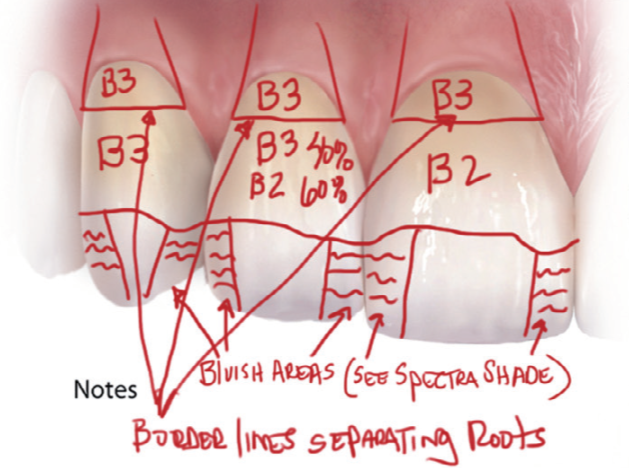
\includegraphics[width=0.5\textwidth]{grafiken/lab_card.png}
			\caption{Cutout of a lab card \citep{sharpling2014}}
	\label{fig:lab_card}
\end{figure}
\bigskip
The Figure \ref{fig:CrownProcesses} shows the sequential states of the dental crowns after each main process conducted by the dental technologist. First of all, the crowns have to be milled out of cylindrical blank which can provide enough bulk material for about 20 crowns. The milled crowns are colored via variety of brushes using  false colored inks to help the dental technician to visually differentiate the colored regions and the inks from each other, which do not possess their final color and have an extremely low contrast so that it is hard process for the human eye to recognize the borders of the different ink applied areas.

\bigskip
\begin{figure}[h]
	\centering
	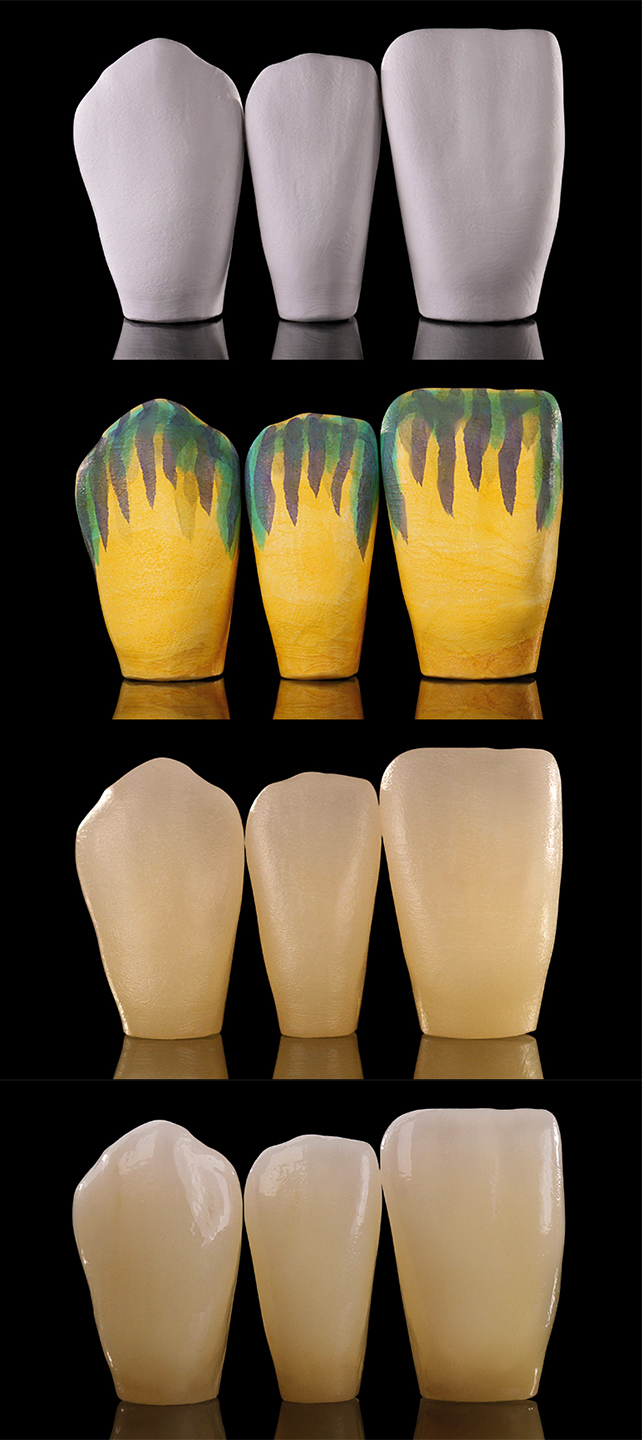
\includegraphics[height=0.6\textwidth]{grafiken/CrownProcesses.jpg}
	\caption{Making of dental implants \citep{zirkonzahn2018} }
	\label{fig:CrownProcesses}
\end{figure} 
 \bigskip

Afterwards the colored dental crowns are sintered for the ceramic to reach its final strength. The false colors of the inks evaporate at temperatures above 1200\textdegree C and the metal-ionic ink becomes more visible providing the zirconia natural tooth like shade which roots from the depths of the ceramic structure. As a final process the crowns are masked and polished.



\chapter{Review of the State of the Research and Technology}
\label{sec:kritik_stand_technik}
The second stage ,the coloring process, is the part which this thesis is focused on. The coloring process is a qualitative procedure. The amount of ink to apply on the dents and edges of the crown are described in measures of brush strokes. The literature or the technical documentation does not provide a quantitative approach about the required amount of ink. In Figure \ref{fig:false_colored} one can observe how cumbersome it is to accomplish the full colorization of a crown. More importantly, if the batch size is large an important problem surfaces. The sequential teeth have to comply with the natural ones already present in the application area or the ones colored before. The shading tolerances cannot be allowed to be too high, because of the uncommon irregularity of the teeth colors this situation would cause.
\bigskip
\begin{figure}[h]
	\centering
	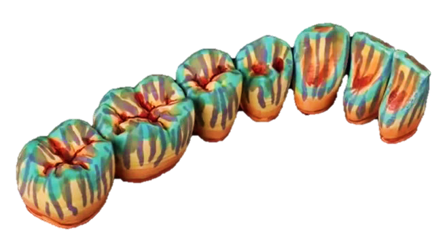
\includegraphics[width=0.6\textwidth]{grafiken/false_colored.png}
	\caption{False colored crowns after manual brushing \citep{zirkonzahn2018}}
	\label{fig:false_colored}
\end{figure}
\bigskip

There are already devices to check the generated shade as a quality control measure. The proactive measure to control the shade to be generated is premixing the coloring agent with the brightener at the factory to guarantee that the zirconia will have the predefined color after the sinter if the zirconia is soaked in to the ink or the ink is applied on the surface until saturation is reached.
For the printing process the amount of ink required for each shade, the time of depletion of the micro drops from the surface of the zirconia in the the porous structure and the size of the generated spot as well as the distribution of the ink depending on the radial distance from the center of the spot is of high interest.